\documentclass[9pt,aspectratio=169,xcolor=table]{beamer}
%~~~~~~~~~~~~~~~~~~~~~~~~~~~~~~~~~~~~~~~~~~~~~~~~~~~~~~~~~~~~~~~~~~~~~~~~~~~~~~
% Use roboto Font (recommended)
\usepackage[sfdefault]{roboto}
\usepackage[utf8]{inputenc}
\usepackage[T1]{fontenc}
%~~~~~~~~~~~~~~~~~~~~~~~~~~~~~~~~~~~~~~~~~~~~~~~~~~~~~~~~~~~~~~~~~~~~~~~~~~~~~~
%~~~~~~~~~~~~~~~~~~~~~~~~~~~~~~~~~~~~~~~~~~~~~~~~~~~~~~~~~~~~~~~~~~~~~~~~~~~~~~
% Define where theme files are located. ('/styles')
\usepackage{styles/fluxmacros}
\usefolder{styles}
% Use Flux theme v0.1 beta
% Available style: asphalt, blue, red, green, gray
\usetheme[style=gray]{flux}
%~~~~~~~~~~~~~~~~~~~~~~~~~~~~~~~~~~~~~~~~~~~~~~~~~~~~~~~~~~~~~~~~~~~~~~~~~~~~~~
%~~~~~~~~~~~~~~~~~~~~~~~~~~~~~~~~~~~~~~~~~~~~~~~~~~~~~~~~~~~~~~~~~~~~~~~~~~~~~~
% Extra packages
\usepackage{booktabs}
\usepackage{colortbl}
\usepackage{ragged2e}
\usepackage{amssymb}
\usepackage{multirow}
\usepackage{tikz}
\usetikzlibrary{arrows.meta, positioning, fit, backgrounds, calc, decorations.pathreplacing}
\setbeamertemplate{itemize items}[square]
\usepackage[scaled=.92]{beramono}
\usepackage{listings}
\usepackage{styles/lstlangarm}
\usepackage{array}
\definecolor{bgcolor}{HTML}{F2E9E9}
% lstlangarm.sty references \color{mauve} for string literals but never defines
% it -- only fires when a listing contains a string. Define it here.
\definecolor{mauve}{rgb}{0.58,0,0.82}
% lstlangarm's C style sets commentstyle=green!20, which is unreadable on the
% pink listing background. Darken it globally.
\lstset{commentstyle=\color{green!45!black}}
% ragged-right fixed-width column -- must be defined in the preamble, never
% inside a frame (\newcolumntype's #1 breaks beamer's frame scanner)
\newcolumntype{R}[1]{>{\RaggedRight\arraybackslash}p{#1}}
%~~~~~~~~~~~~~~~~~~~~~~~~~~~~~~~~~~~~~~~~~~~~~~~~~~~~~~~~~~~~~~~~~~~~~~~~~~~~~~
% Table striping: odd rows white, even rows very light gray.
% Needs \documentclass[...,xcolor=table]{beamer} (beamer loads xcolor itself,
% so the option must go on the class, not \usepackage).
\definecolor{stripe}{gray}{0.94}
% \striped makes body rows alternate white, gray, white, ... starting white.
% \rowcolors counts from the first coloured body row; the header is not counted.
\newcommand{\striped}{\rowcolors{1}{white}{stripe}}
%~~~~~~~~~~~~~~~~~~~~~~~~~~~~~~~~~~~~~~~~~~~~~~~~~~~~~~~~~~~~~~~~~~~~~~~~~~~~~~
%~~~~~~~~~~~~~~~~~~~~~~~~~~~~~~~~~~~~~~~~~~~~~~~~~~~~~~~~~~~~~~~~~~~~~~~~~~~~~~
% TikZ block styles -- matches ch1/ch2
% Colour variables are named identically in the book's stm32primer.tex, so any
% tikzpicture using only the \tikzset{...} styles below can be copied verbatim
% between slides and book. Only the \definecolor/\colorlet VALUES differ: the
% book is printed, so it keeps every stroke pure black with muted fills. These
% slides are projected, so both fill AND stroke are bright and saturated to
% grab attention -- see stm32primer.tex for the print palette.
\definecolor{blkfill}{HTML}{DCEBFF}
\definecolor{blkline}{HTML}{1565C0}
\definecolor{accentfill}{HTML}{FFE0B2}
\definecolor{accentline}{HTML}{E65100}
\definecolor{memfill}{HTML}{DFF5DA}
\definecolor{memline}{HTML}{2E7D32}
\definecolor{cellfill}{HTML}{FFFFFF}
\definecolor{cellline}{HTML}{424242}
\definecolor{bitmaskfill}{HTML}{DCEBFF}
\definecolor{bitmaskline}{HTML}{1565C0}
\definecolor{bithitfill}{HTML}{FFE0B2}
\definecolor{bithitline}{HTML}{E65100}
\tikzset{
  blk/.style   = {rectangle, rounded corners=2pt, draw=blkline, fill=blkfill,
                  thick, align=center, font=\small, minimum height=9mm, inner sep=3pt},
  cpublk/.style= {rectangle, rounded corners=2pt, draw=accentline, fill=accentfill,
                  thick, align=center, font=\small\bfseries, minimum height=9mm, inner sep=3pt},
  memblk/.style= {rectangle, rounded corners=2pt, draw=memline, fill=memfill,
                  thick, align=center, font=\small, minimum height=9mm, inner sep=3pt},
  cell/.style  = {rectangle, draw=cellline, fill=cellfill, align=center,
                  font=\normalsize\ttfamily, minimum height=7mm, inner sep=2pt},
  lbl/.style   = {font=\scriptsize, text=Gray},
  flow/.style  = {-{Stealth[length=2mm]}, thick, draw=blkline},
  busline/.style={thick, draw=cellline},
}
% NOTE (theme quirks -- all fail SILENTLY, always page through the PDF):
%  - a second \\ inside a nested {...} group in a TikZ node breaks parsing
%  - {\small ...} wrapped around a nested itemize eats the frame title + list
%  - \usebeamercolor on a [plain] frame falls through to an unstyled default
%  - \newcolumntype inside a frame breaks beamer's frame scanner
%  - lstlisting needs \begin{frame}[fragile]
%  - a TikZ picture wider than its column silently overflows into neighbours
%~~~~~~~~~~~~~~~~~~~~~~~~~~~~~~~~~~~~~~~~~~~~~~~~~~~~~~~~~~~~~~~~~~~~~~~~~~~~~~
%%%%%%%%%%%%%%%%%%%%%%%%%%%%%%%%%%%
%% BEGIN CONDITIONAL COMPILATION %%
%%%%%%%%%%%%%%%%%%%%%%%%%%%%%%%%%%%
\newif\ifwebex
%\webextrue % uncomment to generate section separator
\ifwebex
\AtBeginSection[]{
  \begin{frame}
  \vfill
  \centering
  \begin{beamercolorbox}[sep=8pt,center,shadow=true,rounded=true]{title}
    \usebeamerfont{title}\insertsectionhead\par%
  \end{beamercolorbox}
  \vfill
  \end{frame}
}
\else
\AtBeginSection[]
{
{
    \setbeamercolor{background canvas}{bg=yellow!10}
    \begin{frame}[plain]
        \frametitle{Table of Contents}
        \tableofcontents[currentsection]
    \end{frame}
}
}
\fi
%%%%%%%%%%%%%%%%%%%%%%%%%%%%%%%%%%%
%% END CONDITIONAL COMPILATION   %%
%%%%%%%%%%%%%%%%%%%%%%%%%%%%%%%%%%%
%~~~~~~~~~~~~~~~~~~~~~~~~~~~~~~~~~~~~~~~~~~~~~~~~~~~~~~~~~~~~~~~~~~~~~~~~~~~~~~
% Information
\title{The ARM Cortex-M4 Programmer's Model}
\subtitle{\emph{Introduction to ARM Cortex-M Microprocessors} --- Chapter 2}
\author{Mun\'{i}m Zabidi}
\institute{\color{primary}Faculty of Electrical Engineering, Universiti Teknologi Malaysia}
\date{\today}
\titlegraphic{assets/logoutmwhite.png}
%~~~~~~~~~~~~~~~~~~~~~~~~~~~~~~~~~~~~~~~~~~~~~~~~~~~~~~~~~~~~~~~~~~~~~~~~~~~~~~
\begin{document}
\titlepage
\begin{frame}{Table of Contents}
    \tableofcontents
\end{frame}

%===============================================================================
\section{Why This Matters}
%===============================================================================
\begin{frame}{Why This Chapter Matters}
    \leavevmode
    The previous chapter introduced a generic processor. To write real programs, we need to know one specific processor in detail: how many registers it has, what they are called, which ones have a special meaning, and how it stores the result of a comparison.

    This detailed view is called the \emph{programmer's model}. It is the part of the hardware that software can actually see. Everything you write, in assembly or in C, works by using the small set of registers this chapter describes.
\end{frame}

\begin{frame}{Objectives}
    \leavevmode
    {\small After completing this chapter, you should be able to:}
    \vspace{2mm}
    {\small
    \begin{enumerate}\itemsep2pt
        \item Distinguish instruction set architecture, microarchitecture, and platform architecture, and give one meaning of ``32-bit'' under each layer.
        \item State the defining characteristics of a RISC load-store architecture and contrast them with CISC.
        \item Explain how a pipeline raises throughput, and why a short pipeline suits an embedded processor.
        \item Select the appropriate ARM Cortex profile (A, R, or M) for a given application.
        \item Name the Cortex-M4 core registers R0--R15 and state the special role of SP, LR, and PC.
        \item Interpret the N, Z, C, and V flags of the APSR after an arithmetic operation.
        \item Describe the layout of the Cortex-M 4\,GB memory map and identify which region holds code, variables, and peripherals.
        \item Explain little-endian byte ordering and distinguish the AHB and APB buses by the peripherals each one serves.
    \end{enumerate}}
\end{frame}

%===============================================================================
\section{Architecture and Organization}
%===============================================================================
\begin{frame}{Three Layers Called ``Architecture''}
    \leavevmode
    \begin{center}
    {\small
    \striped
    \begin{tabular}{@{}l R{.58\textwidth}@{}}
        \toprule
        \textbf{Layer} & \textbf{What it specifies} \\
        \midrule
        \textbf{Instruction Set}\newline\textbf{Architecture (ISA)}
            & The language the processor understands: instruction formats,
              register set, addressing modes. Visible to an assembly programmer.
              \emph{x86, ARM, RISC-V} \\[2mm]
        \textbf{Microarchitecture}
            & How that ISA is implemented in silicon: control signals, cache
              size, pipeline depth, ALU internals \\[2mm]
        \textbf{Platform}\newline\textbf{architecture}
            & How the processor reaches the rest of the system: buses, memory controllers,
              DMA. \emph{ARM's AMBA} \\
        \bottomrule
    \end{tabular}}
    \end{center}
    \vspace{2mm}
    \begin{block}{These layers are independent}
        One ISA can be built by many different microarchitectures. This is why code written for one ISA can run on physically different chips. It is the commercial foundation of the whole ARM ecosystem.
        \vspace{1mm}
        The term ``32-bit'' can describe the ISA, the ALU width, or the address bus. On the Cortex-M4, these three meanings happen to be the same. But they are still three separate, independent facts.
    \end{block}
\end{frame}

\begin{frame}{Von Neumann Architecture}
    \begin{columns}[c]
    \begin{column}{.42\textwidth}
        \begin{center}
        \begin{tikzpicture}[x=10mm, y=10mm]
            \node[cpublk, minimum width=20mm, minimum height=30mm] (cpu) at (0,0) {CPU};
            \node[memblk, minimum width=20mm, minimum height=30mm] (mem) at (3.6,0) {Code\\+\\Data\\Memory};
            % one shared bus: three lines, one label on the middle one
            \draw[busline, line width=1.2pt, draw=secondary]
                  ([yshift=4mm]cpu.east) -- ([yshift=4mm]mem.west);
            \draw[busline, line width=1.2pt, draw=primary]
                  (cpu.east) -- (mem.west);
            \draw[busline, line width=1.2pt, draw=Gray]
                  ([yshift=-4mm]cpu.east) -- ([yshift=-4mm]mem.west);
            \node[lbl, anchor=north] at (1.8,-0.62) {one shared bus};
        \end{tikzpicture}
        \end{center}
    \end{column}
    \begin{column}{.56\textwidth}
        \begin{itemize}
            \item A \alert{single} storage system holds both program and data.
            \item An instruction typically needs \alert{two clock cycles}: one to fetch the instruction, another to fetch its data.
            \item Instruction and data cannot travel at the same time, since they share one bus.
            \item Simple and inexpensive, but the shared bus quickly becomes a bottleneck.
        \end{itemize}
    \end{column}
    \end{columns}
    \vspace{2mm}
    {\small This shared-bus limit is called the \alert{Von Neumann bottleneck}. The next slide shows an architecture built to remove it.}
\end{frame}

\begin{frame}{Harvard Architecture}
    \begin{columns}[c]
    \begin{column}{.46\textwidth}
        \begin{center}
        \begin{tikzpicture}[x=10mm, y=10mm]
            \node[cpublk, minimum width=20mm, minimum height=30mm] (cpu)  at (0,0) {CPU};
            \node[memblk, minimum width=20mm, minimum height=11mm] (code) at (3.6,0.95)  {Code\\Memory};
            \node[memblk, minimum width=20mm, minimum height=11mm] (data) at (3.6,-0.95) {Data\\Memory};
            % buses run due east-west; labels sit on the line with a white gap
            \draw[busline, line width=1.2pt, draw=secondary]
                  (cpu.east |- code) -- node[lbl, fill=white, inner sep=1.5pt,
                  text=secondary] {bus 1} (code.west);
            \draw[busline, line width=1.2pt, draw=primary]
                  (cpu.east |- data) -- node[lbl, fill=white, inner sep=1.5pt,
                  text=primary] {bus 2} (data.west);
        \end{tikzpicture}
        \end{center}
    \end{column}
    \begin{column}{.52\textwidth}
        \begin{itemize}
            \item \alert{Two separate memories} for program and data, each with its own bus.
            \item With pipelining, an instruction can complete in \alert{one cycle}: the next instruction is fetched while the current one reads its data.
            \item Most modern architectures are Harvard, or a close variant of it.
        \end{itemize}
    \end{column}
    \end{columns}
    \vspace{2mm}
    \begin{block}{What the Cortex-M4 actually is}
        A \alert{modified Harvard} machine. It has separate instruction and data buses (three AHB-Lite interfaces), but a \alert{single unified address space}. You get the speed of Harvard, but you can still load a constant stored in flash with an ordinary load instruction.
    \end{block}
\end{frame}

\begin{frame}{CISC vs RISC}
    \begin{center}
    \striped
    \begin{tabular}{p{.44\textwidth}p{.44\textwidth}}
        \toprule
        \textbf{CISC} & \textbf{RISC} \\
        \midrule
        Emerged when memory was expensive and compilers were primitive & Deliberately simplified so that hardware is fast and \alert{predictable} \\
        Complex hardware instruction decoder & Relies heavily on the compiler for optimisation \\
        Variable-length instructions, multi-clock operations & Uniform-length instructions, single-cycle operations, simple pipelining \\
        \alert{Memory-to-memory}: arithmetic can operate directly on memory & \alert{Register-to-register}: memory is reached only via explicit load and store \\
        Dense code, but more cycles per instruction & More instructions, but far fewer cycles per instruction \\
        e.g.\ Intel x86, AMD & e.g.\ ARM, RISC-V \\
        \bottomrule
    \end{tabular}
    \end{center}
    \vspace{3mm}
    \begin{block}{Complexity does not disappear --- it moves}
        RISC moves complexity out of the hardware decoder and into the compiler. The result is a set of simple instructions that pipeline cleanly, and behave in a predictable way.
    \end{block}
\end{frame}

\begin{frame}[fragile]{Memory Access vs.\ Register Architecture}
	\begin{columns}[T]
		\begin{column}{.48\textwidth}
			\begin{minipage}[t][.28\textheight][t]{\linewidth}
				\textbf{CISC} --- Memory-to-Memory
				\begin{itemize}
					\item Memory operations are embedded in arithmetic instructions.
					\item A single instruction can load from memory, compute, and write the result back.
				\end{itemize}
			\end{minipage}

			{\small\color{red!75!black}
				\begin{verbatim}
					; x = x + 1
					ADD [eax], ebx
			\end{verbatim}}
		\end{column}
		\begin{column}{.48\textwidth}
			\begin{minipage}[t][.28\textheight][t]{\linewidth}
				\textbf{RISC} --- Register-to-Register
				\begin{itemize}
					\item Strict load-store architecture.
					\item Memory is accessed only by dedicated \texttt{LDR} and \texttt{STR} instructions.
				\end{itemize}
			\end{minipage}

			{\small\color{red!75!black}
				\begin{verbatim}
					; x = x + 1
					LDR r0, [r1]   ; load into register
					ADD r0, r0, r2 ; register arithmetic
					STR r0, [r1]   ; store back to memory
			\end{verbatim}}
		\end{column}
	\end{columns}
\end{frame}

\begin{frame}{The Load-Store Principle}
    \leavevmode
    \begin{center}
    \fbox{\parbox{.8\textwidth}{\centering\vspace{1mm}
    \textbf{Key idea:} the ALU never operates directly on memory. Data must first move into a register.
    \vspace{1mm}}}
    \end{center}
    \vspace{2mm}
    \begin{center}
    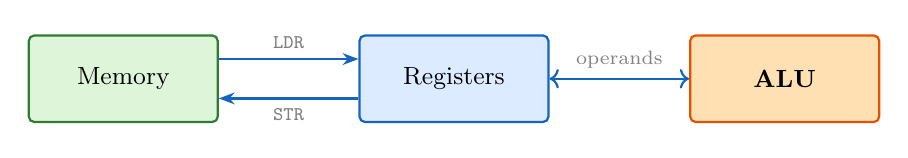
\begin{tikzpicture}[x=10mm, y=10mm]
        \node[memblk, minimum width=24mm, minimum height=11mm] (mem) at (0,0)   {Memory};
        \node[blk,    minimum width=24mm, minimum height=11mm] (reg) at (4.2,0) {Registers};
        \node[cpublk, minimum width=24mm, minimum height=11mm] (alu) at (8.4,0) {ALU};
        \draw[flow] ([yshift=2.5mm]mem.east) -- node[lbl, above] {\texttt{LDR}} ([yshift=2.5mm]reg.west);
        \draw[flow] ([yshift=-2.5mm]reg.west) -- node[lbl, below] {\texttt{STR}} ([yshift=-2.5mm]mem.east);
        \draw[flow, <->] (reg.east) -- node[lbl, above] {operands} (alu.west);
    \end{tikzpicture}
    \end{center}
    \vspace{1mm}
    {\small\centering \texttt{LDR} $\to$ ALU operation $\to$ \texttt{STR}: this is the \alert{only} way the ALU ever touches memory. Even \texttt{x = x + 1;} costs \alert{three} instructions, never one. This pattern shapes every assembly example in Chapters~5 and~6.\par}
    \vspace{1mm}
    {\small \textbf{Digital-electronics connection:} registers sit only a few gate delays from the ALU. Memory sits across a bus, with address decoding and longer settling times. Forcing operands through registers first is what lets the clock run fast.}
\end{frame}

\begin{frame}[plain]{Pipelining}
    \leavevmode
    Doing fetch, decode, and execute strictly one after another \alert{wastes hardware}. While the ALU is busy, the fetch unit sits idle, doing nothing.

    A \alert{pipeline} overlaps these stages instead, like doing laundry: you do not wait for one load to finish drying before starting to wash the next one.
    \vspace{2mm}
    \begin{center}
    \begin{tikzpicture}[x=15mm, y=8mm]
        \tikzset{
          stage/.style = {rectangle, draw=Gray, thick, rounded corners=2pt,
                          minimum width=13mm, minimum height=6.5mm,
                          font=\small, inner sep=1pt},
          fetch/.style = {stage, fill=secondary!12},
          dec/.style   = {stage, fill=white},
          exec/.style  = {stage, draw=primary, fill=primary!12},
        }
        \foreach \c in {1,...,5}{
          \node[font=\small\bfseries] at (\c,1.25) {Cycle \c};
        }
        \foreach \r/\start in {1/1, 2/2, 3/3}{
          \pgfmathsetmacro{\y}{0.5-(\r-1)*0.95}
          \node[anchor=east, font=\small] at (0.45,\y) {Instruction \r};
          \pgfmathtruncatemacro{\cf}{\start}
          \pgfmathtruncatemacro{\cd}{\start+1}
          \pgfmathtruncatemacro{\ce}{\start+2}
          \node[fetch] at (\cf,\y) {Fetch};
          \node[dec]   at (\cd,\y) {Decode};
          \node[exec]  at (\ce,\y) {Execute};
        }
        \draw[dashed, thick, draw=primary] (2.5,0.95) -- (2.5,-1.9);
        \node[anchor=north, font=\scriptsize\itshape, text=primary]
             at (3.75,-1.95) {pipeline full --- one instruction completes every cycle};
    \end{tikzpicture}
    \end{center}
    \vspace{2mm}
    \begin{itemize}
        \item Each instruction still takes three cycles. But once the pipeline is full, \alert{one instruction finishes every cycle}. The Cortex-M4 uses a three-stage pipeline with branch speculation.
        \item RISC instructions are simpler, so they are much easier to build a pipeline for.
    \end{itemize}
\end{frame}

\begin{frame}{What a Pipeline Costs}
    \begin{columns}[T]
    \begin{column}{.48\textwidth}
        \textbf{The PC runs ahead}
        \vspace{1mm}
        {\small While instruction~1 executes, instruction~2 is decoding, and instruction~3 has already been fetched. So the PC does not point at the instruction currently executing.}
        \vspace{2mm}
        {\small This is why \texttt{MOV R0, PC} returns an address four bytes ahead of the current instruction.}
    \end{column}
    \begin{column}{.48\textwidth}
        \textbf{Branches cost more}
        \vspace{1mm}
        {\small When a branch is taken, the instructions already fetched behind it are wrong. The pipeline must be cleared and refilled.}
        \vspace{2mm}
        {\small A three-stage pipeline loses only a few cycles. A long pipeline loses many more.}
    \end{column}
    \end{columns}
    \vspace{3mm}
    \begin{block}{A deliberate design decision}
        A Cortex-A core uses a long pipeline for high peak speed. But a mispredicted branch is expensive there, and how expensive depends on the data.

        The Cortex-M gives up some peak speed on purpose, so its worst-case timing stays close to its average-case timing. Chapter~1 called this property essential for embedded systems.
    \end{block}
\end{frame}

\begin{frame}{More Instructions Does Not Mean Slower}
    \begin{center}
    \fbox{\parbox{.86\textwidth}{\centering\vspace{1mm}
    CPU time $=$ Instruction Count $\times$ Cycles per Instruction $\times$ Clock period
    \vspace{1mm}}}
    \end{center}
    \vspace{4mm}
    \begin{center}
    {\small
    \striped
    \begin{tabular}{@{}l l l@{}}
        \toprule
        \textbf{Term} & \textbf{RISC effect} & \textbf{Why} \\
        \midrule
        Instruction count & \alert{Higher} & More, simpler instructions per task \\
        Cycles per instruction & \alert{Lower} & Each instruction finishes in one cycle \\
        Clock period & \alert{Lower} & A simple decoder permits a faster clock \\
        \bottomrule
    \end{tabular}}
    \end{center}
    \vspace{3mm}
    {\small The product of all three terms is what matters in the end. RISC improves two of the three terms, which is why it usually wins.}
\end{frame}


%===============================================================================
\section{ARM and the Cortex Profiles}
%===============================================================================
\begin{frame}{A Short History of ARM}
    {\small\centering\emph{So why did ARM choose this approach?} To understand the Cortex-M4, we first look at where ARM came from, and how its processor families grew.\par}
    \vspace{2mm}
    \begin{columns}[T]
    \begin{column}{.48\textwidth}
        \begin{itemize}
            \item \textbf{1980s} --- Acorn Computers in Cambridge builds the \textbf{BBC Micro} around the 6502, for the BBC's computer-literacy project.
            \item \textbf{1985} --- Sophie Wilson and Steve Furber design a new CPU: the \alert{Acorn RISC Machine}. The ARM1 has only 24\,800 transistors and uses under 100\,mW.
            \item \textbf{1990} --- ARM Ltd is spun out, jointly owned by Acorn, Apple, and VLSI. ``Acorn'' becomes \alert{Advanced RISC Machines}.
        \end{itemize}
    \end{column}
    \begin{column}{.48\textwidth}
        \begin{itemize}
            \item \textbf{1993} --- The Apple Newton ships with an ARM610. The product itself sells poorly, but the partnership pushes ARM toward a pure licensing model.
            \item \textbf{2000s} --- Mobile phones make ARM the default choice: low power, good enough performance, and easy to license.
            \item \textbf{Today} --- The most widely used ISA on Earth, used in everything from tiny sensors to Apple's M-series chips and Amazon's Graviton servers.
        \end{itemize}
    \end{column}
    \end{columns}
    \vspace{2mm}
    \begin{block}{The pattern worth noticing}
        ARM was designed to be small because Acorn was a small company with a limited budget. That early constraint later became the reason ARM came to dominate the embedded and mobile markets. This is the same cost-and-power argument as in Chapter~1.
    \end{block}
\end{frame}

\begin{frame}{ARM Does Not Make Chips}{Why there is an ST logo on an ARM core}
    \begin{columns}[c]
    \begin{column}{.42\textwidth}
        \begin{center}
        \includegraphics[width=\textwidth, height=.66\textheight, keepaspectratio]%
            {assets/arm-in-soc.png}
        \end{center}
    \end{column}
    \begin{column}{.54\textwidth}
        ARM is \alert{fabless}: it designs processor cores and licenses the design to others. It owns no chip factory itself.
        \vspace{2mm}
        \begin{itemize}
            \item \textbf{Core licence} --- A chip maker puts an ARM core into its own design, then adds its own memory, peripherals, and analog circuits (ST, NXP, Microchip, Nordic, \ldots).
            \item \textbf{Architecture licence} --- A company designs its \emph{own} core that still runs the ARM instruction set. Fewer than ten such licences exist. Apple's M-series is one example.
        \end{itemize}
        \vspace{2mm}
        {\small On your bench: ARM designed the \alert{Cortex-M4 core}. \alert{ST} added the flash, SRAM, GPIO, timers, ADC, and UART around it. The finished product is the \textbf{STM32F446RE}.}
    \end{column}
    \end{columns}
    \vspace{2mm}
    \begin{block}{The hierarchy to keep straight}
        {\small \textbf{ARM} defines the instruction-set architecture and licenses cores. \textbf{Cortex} names families of processor cores built around it. For embedded systems, the family we use is \alert{Cortex-M}.}
    \end{block}
\end{frame}

%\begin{frame}[plain]{ARM Cortex: Three Profiles}
%    \begin{center}
%    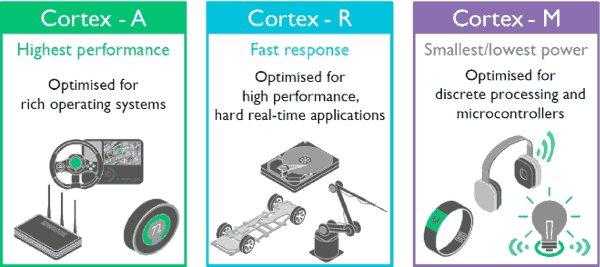
\includegraphics[width=.92\textwidth]{assets/arm-diverse-architecture.png}
%    \end{center}
%    \vspace{1mm}
%    {\small\centering ARM organises its cores into three profiles. This course uses \alert{Cortex-M}; everything that follows applies specifically to that profile.\par}
%\end{frame}

\begin{frame}{The Three Cortex Profiles}
	\begin{center}
		{\small
			\striped
			\begin{tabular}{@{}l R{.24\textwidth} R{.24\textwidth} R{.24\textwidth}@{}}
				\toprule
				& \textbf{Cortex-A} & \textbf{Cortex-R} & \textbf{Cortex-M} \\
				\midrule
				Profile & Application --- highest performance & Real-time --- fast response & Microcontroller --- smallest, lowest power \\
				OS & Linux, Android & RTOS & Bare metal / RTOS \\
		        Instruction set  & 64-bit, 32-bit, Thumb & 32-bit, Thumb & Thumb only \\
				Interrupts  & Software-managed & Deterministic, software-managed & Hardware-managed \\
				Pipeline & Long & Long to medium & {Short} \\
				Cache & Multi-level & Yes & {None} \\
				Found in & Phones, tablets, servers & Storage, industrial, automotive & IoT, sensors, control \\
				\bottomrule
		\end{tabular}}
	\end{center}
	\vspace{3mm}
	\begin{block}{Cortex-M trades peak speed for predictable, low-power execution}
    {\small A short pipeline and no cache mean an instruction takes exactly the time the documentation says it takes. This is the property we said was essential for embedded systems.}
	\end{block}
	\vspace{1mm}
	{\small\centering So where does the Cortex-M4 fit inside the Cortex-M family? That is next.\par}
\end{frame}

\begin{frame}{The Cortex-M Family}
	\begin{center}
		{\small
			\striped
			\begin{tabular}{lp{.72\textwidth}}
				\toprule
				\textbf{Processor} & \textbf{Description} \\
				\midrule
				Cortex-M0  & Very small (from 12K gates), lowest cost, ultra-low power \\
				Cortex-M0+ & Most energy-efficient; adds single-cycle I/O and vector-table relocation \\
				Cortex-M3  & Rich instruction set, hardware divide, MAC, full debug and trace \\
				\alert{Cortex-M4} & {Everything in the M3, plus DSP (SIMD, fast MAC) and an optional
					single-precision FPU} \\
				Cortex-M7  & High performance, dual-issue pipeline, optional double-precision FPU, cache and TCM \\
				Cortex-M23 & ARMv8-M Baseline with TrustZone; ultra-low-power secure IoT \\
				Cortex-M33 & ARMv8-M Mainline with TrustZone, optional DSP/FPU; widely used secure MCU core \\
				Cortex-M35P & Like M33 but with built-in physical tamper resistance \\
				Cortex-M52 & Smallest core with Arm Helium (MVE); efficient ML/DSP for cost-sensitive designs \\
				Cortex-M55 & First Helium core; strong scalar + vector (ML/DSP) performance \\
				Cortex-M85 & Highest-performance Cortex-M; superscalar + Helium, strongest ML/DSP and security features \\
				\bottomrule
		\end{tabular}}
	\end{center}
	\vspace{2mm}
	{\small The \textbf{F} in STM32F446RE's core name --- Cortex-M4\alert{F} --- shows that a floating-point unit is fitted. Your board can therefore do single-precision floating-point arithmetic in hardware.}
\end{frame}
\begin{frame}[plain]{Inside the Cortex-M4}
	\begin{columns}[c]
		\begin{column}{.40\textwidth}
			\begin{center}
				\includegraphics[width=\linewidth, height=.78\textheight, keepaspectratio]%
				{assets/m4-simple-block.png}
			\end{center}
		\end{column}
		\begin{column}{.55\textwidth}
			\textbf{What each block is for}
			\begin{itemize}
				\item \textbf{CPU (Armv7-M)} --- the datapath from Chapter~1, now with 16 registers.
				\item \textbf{NVIC} --- Nested Vectored Interrupt Controller. Interrupts are managed in hardware (Chapter~9).
				\item \textbf{DSP / FPU} --- SIMD operations, fast multiply-accumulate, and single-precision floating-point.
				\item \textbf{MPU} --- Memory Protection Unit.
				\item \textbf{3\,$\times$ AHB-Lite} --- the separate instruction and data buses that give the core its modified-Harvard design.
				\item \textbf{JTAG / Serial Wire, ITM/ETM} --- the debug and trace hardware your ST-LINK talks to.
			\end{itemize}
		\end{column}
	\end{columns}
\end{frame}

\begin{frame}[plain]{Cortex-M4 Features}{The specification, in one place}
	\begin{columns}[c]
		\begin{column}{.55\textwidth}
			{\small
				\begin{tabular}{@{}r|p{.95\linewidth}@{}}
					\textbf{Architecture} & ARMv7E-M \\
					\textbf{ISA} & Thumb-2 \\
					\textbf{Pipeline} & 3-stage + branch speculation \\
					\textbf{Bus interface} & 3 $\times$ AMBA AHB-Lite \\
					\textbf{DSP} & Single-cycle 16/32-bit MAC \\
					& Single-cycle dual 16-bit MAC \\
					& 8/16-bit SIMD arithmetic \\
					& Hardware divide (2--12 cycles) \\
					\textbf{Floating point} & Single precision, IEEE 754 \\
					\textbf{Interrupts} & Nested Vectored Interrupt Controller \\
					& Non-maskable interrupt (NMI) \\
					& 1 to 240 physical interrupts \\
					& 8 to 256 priority levels \\
					\textbf{HLL support} & Designed to be programmed fully in C \\
			\end{tabular}}
		\end{column}
		\begin{column}{.40\textwidth}
			\begin{center}
				\includegraphics[width=\linewidth, height=.78\textheight, keepaspectratio]%
				{assets/m4-simple-block.png}
			\end{center}
		\end{column}
	\end{columns}
	\vspace{1mm}
	{\small Every row above has already appeared in this chapter, except the last one. That last row is the reason Chapter~4 is written in C, not assembly.\par}
\end{frame}

\begin{frame}{Memory-Mapped I/O}{The idea the rest of the course rests on}
    \begin{block}{There is no special instruction for I/O}
        A peripheral register is just an address. You turn an LED on with the same \texttt{STR} instruction you use to write to a variable. Only the address is different.
    \end{block}
    \vspace{3mm}
    \begin{center}
    \striped
    \begin{tabular}{lll}
        \toprule
        \textbf{What you write in C} & \textbf{What it becomes} & \textbf{Where it lands} \\
        \midrule
        \texttt{c = a + b;}              & \texttt{STR R2, [R3]} & SRAM, \texttt{0x2000\,xxxx} \\
        \texttt{GPIOA->ODR |= (1<<5);}   & \texttt{STR R2, [R3]} & \alert{peripheral}, \texttt{0x4002\,0014} \\
        \bottomrule
    \end{tabular}
    \end{center}
    \vspace{3mm}
    {\small Same instruction, same registers, different address. And one of those addresses lights a real LED on \texttt{PA5}. That is the whole trick. Chapter~8 is where you put it to use.}
\end{frame}

%===============================================================================
\section{STM32: The Chip and the Boards}
%===============================================================================
\begin{frame}{From ARM to the Board on Your Desk}
    \leavevmode
    Four names are easy to confuse: ARM, Cortex-M4, STM32, Nucleo. Each name is a different layer of the same stack.

    \vspace{3mm}
    \begin{center}
    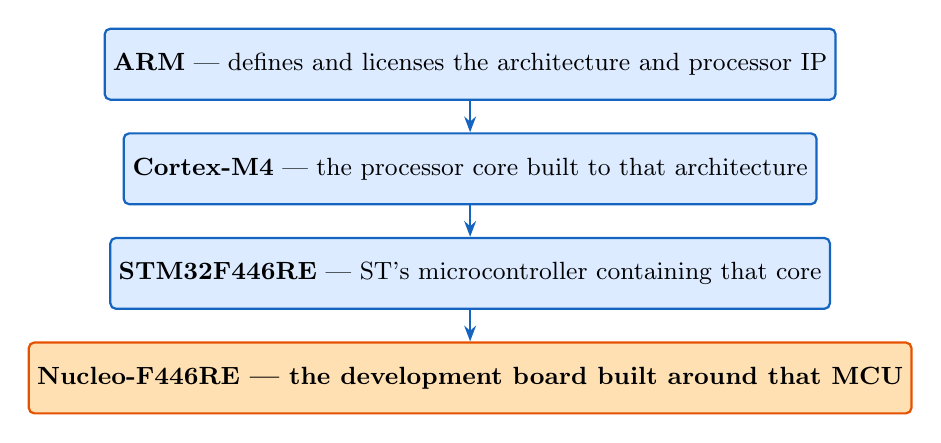
\begin{tikzpicture}[node distance=4mm]
        \node[blk,    minimum width=88mm] (arm)    {\textbf{ARM} --- defines and licenses the architecture and processor IP};
        \node[blk,    minimum width=88mm, below=of arm]    (cortex) {\textbf{Cortex-M4} --- the processor core built to that architecture};
        \node[blk,    minimum width=88mm, below=of cortex] (stm32)  {\textbf{STM32F446RE} --- ST's microcontroller containing that core};
        \node[cpublk, minimum width=88mm, below=of stm32]  (nucleo) {\textbf{Nucleo-F446RE} --- the development board built around that MCU};
        \foreach \a/\b in {arm/cortex, cortex/stm32, stm32/nucleo}{\draw[flow] (\a) -- (\b);}
    \end{tikzpicture}
    \end{center}

    \vspace{2mm}
    {\small\centering Every slide from here on sits at one of these four levels. Keeping them separate is the best way to avoid confusing ``ARM,'' ``the chip,'' and ``the board.''\par}
\end{frame}

\begin{frame}{What Is an STM32?}
    \begin{block}{STM32}
        \textbf{ST}Microelectronics' family of \textbf{32}-bit microcontrollers, each built around a licensed \alert{ARM Cortex-M} core.
    \end{block}
    \vspace{2mm}
    \begin{columns}[T]
    \begin{column}{.46\textwidth}
        \textbf{ARM supplies the core}
        \begin{itemize}
            \item The Cortex-M4 datapath, registers, and instruction set: everything covered so far in this chapter.
            \item The same core, across every vendor's chips.
        \end{itemize}
        \vspace{1mm}
        {\small So Cortex-M4 code can move between different chips, at the core level.}
    \end{column}
    \begin{column}{.5\textwidth}
        \textbf{ST adds everything else}
        \begin{itemize}
            \item Flash and SRAM, in specific sizes
            \item Peripherals: GPIO, timers, ADC, DAC, UART, SPI, I\textsuperscript{2}C, CAN, USB
            \item Clock tree, power management, packaging
        \end{itemize}
        \vspace{1mm}
        {\small These parts are \alert{not} portable. They are ST's own design. Chapters~8--13 focus on programming them.}
    \end{column}
    \end{columns}
    \vspace{2mm}
    {\small The family covers many market needs: \textbf{F} (general purpose), \textbf{L} (low power), \textbf{G} (advanced general purpose), \textbf{H} (high performance), \textbf{WB} (wireless), \textbf{U} (ultra-low power). We use an \alert{STM32F4}.}
\end{frame}

\begin{frame}[plain]{Reading the Part Number}{Every character means something}
    \begin{center}
    \includegraphics[height=.6\textheight, keepaspectratio]%
        {assets/stm32-naming.png}
    \end{center}
    \vspace{1mm}
    \begin{center}
    {\small
    \begin{tabular}{@{}ccccccc@{}}
        \textbf{STM32} & \textbf{F} & \textbf{446} & \textbf{R} & \textbf{E} &
        \textbf{T} & \textbf{6} \\
        32-bit MCU & Foundation & high perf.\ + & 64 pins & 512\,KB &
        plastic & $-40$ to \\
                   &            & DSP with FPU &        & flash   & TQFP   & $+85\,^\circ$C \\
    \end{tabular}}
    \end{center}
    \vspace{1mm}
    {\small\centering A part number is a specification. It is not a serial number.\par}
\end{frame}

\begin{frame}[plain]{The Chip Itself}{STM32F446RE in LQFP64}
    \begin{columns}[c]
    \begin{column}{.5\textwidth}
        \begin{center}
        \includegraphics[width=\textwidth, height=.76\textheight, keepaspectratio]%
            {assets/f446-lqfp64.png}
        \end{center}
    \end{column}
    \begin{column}{.46\textwidth}
        \textbf{STM32F446RE}
        \begin{itemize}
            \item Core: ARM Cortex-M4
            \item Clock: up to 180\,MHz
            \item Flash: 512\,KB
            \item SRAM: 128\,KB
            \item FPU and DSP: single-precision floating-point and DSP instructions for real-time work
            \item Rich peripheral set: GPIO, timers, UART, I\textsuperscript{2}C, SPI, CAN, USB
        \end{itemize}
        \vspace{2mm}
        {\small \textbf{R} = 64 pins and \textbf{T} = LQFP, exactly as the part number said two slides ago.}
    \end{column}
    \end{columns}
\end{frame}

\begin{frame}[plain]{STM32 Boards}{The three you will actually use}
	\begin{columns}[T]
		\begin{column}{.32\textwidth}
			\begin{minipage}[c][.48\textheight][c]{\linewidth}
				\centering
				\includegraphics[width=\linewidth, keepaspectratio]%
				{assets/NUCLEO-F446RE.jpg}
			\end{minipage}
			\vspace{1mm}
			\centering\textbf{Nucleo-F446RE}
			{\small
				\begin{itemize}\itemsep0pt
					\item Our running board all semester
					\item ST-LINK built in --- no separate debugger needed
					\item Arduino Uno pinout \(+\) morpho headers
			\end{itemize}}
		\end{column}
		\begin{column}{.32\textwidth}
			\begin{minipage}[c][.48\textheight][c]{\linewidth}
				\centering
				\includegraphics[width=.85\linewidth, keepaspectratio]%
				{assets/blue_pill.jpg}
			\end{minipage}
			\vspace{1mm}
			\centering\textbf{Blue Pill}
			{\small
				\begin{itemize}\itemsep0pt
					\item Not made by ST; one of many third-party boards
					\item Cheapest way to get a Cortex-M4 on a breadboard
					\item Debugger \alert{not} included --- needs the ST-LINK
			\end{itemize}}
		\end{column}
		\begin{column}{.32\textwidth}
			\begin{minipage}[c][.48\textheight][c]{\linewidth}
				\centering
				\includegraphics[width=.6\linewidth, keepaspectratio]%
				{assets/st-link-v2.jpg}
			\end{minipage}
			\vspace{1mm}
			\centering\textbf{ST-LINK V2}
			{\small
				\begin{itemize}\itemsep0pt
					\item External programmer/debugger over SWD
					\item What the Blue Pill needs; the Nucleo has one built in
					\item Same tool, same workflow, either board
			\end{itemize}}
		\end{column}
	\end{columns}
	\vspace{2mm}
	{\small\centering Same Cortex-M4 core, same ISA, but very different boards.\par}
\end{frame}

\begin{frame}{The Nucleo-F446RE Board}{What ST adds around the chip}
    \begin{columns}[c]
    \begin{column}{.48\textwidth}
        \begin{center}
        \includegraphics[width=\textwidth, height=.62\textheight, keepaspectratio]%
            {assets/nucleo-annotated.png}
        \end{center}
    \end{column}
    \begin{column}{.48\textwidth}
        The Nucleo board adds four useful features that make experiments easy:
        \begin{itemize}
            \item \alert{ST-Link debugger} --- the detachable top section. One USB cable supplies power, programming, and debugging. No separate programmer is needed.
            \item \alert{User button and LED} --- \texttt{PC13} and \texttt{PA5}. Enough to check a program works, with no external wiring.
            \item \alert{Arduino connector} --- accepts standard off-the-shelf shields.
            \item \alert{Morpho connector} --- brings out every STM32 pin, including the ones the Arduino header cannot reach.
        \end{itemize}
    \end{column}
    \end{columns}
    \vspace{1mm}
    {\small Full details are in the \emph{STM32 Nucleo-64 Boards User Manual} (UM1724).\par}
\end{frame}

\begin{frame}[plain]{Nucleo-F446RE Pinout}
    \begin{columns}[c]
    \begin{column}{.5\textwidth}
        \begin{center}
        \includegraphics[width=\textwidth, height=.74\textheight, keepaspectratio]%
            {assets/nucleo-pinout.png}
        \end{center}
    \end{column}
    \begin{column}{.46\textwidth}
        Two connector systems share the board:
        \vspace{2mm}
        \begin{itemize}
            \item \alert{Arduino} headers (CN5--CN10, magenta) --- \texttt{D0--D15}, \texttt{A0--A5}. Accept standard shields.
            \item \alert{Morpho} headers (CN7, CN10, blue) --- every STM32 pin, including the ones the Arduino header leaves out.
        \end{itemize}
        \vspace{3mm}
        {\small Pins used throughout the course:\\
        \texttt{PA5} --- user LED \quad(Arduino \texttt{D13})\\
        \texttt{PC13} --- user button}
    \end{column}
    \end{columns}
\end{frame}


%===============================================================================
\section{Cortex-M4 Programmer's Model}
%===============================================================================
\begin{frame}{Now: The Programmer's View}
    \leavevmode
    \begin{center}
    \fbox{\parbox{.8\textwidth}{\centering\vspace{1mm}
    We move from processor \emph{architecture} to the processor's \emph{programmer's model}.
    \vspace{1mm}}}
    \end{center}

    \vspace{3mm}
    {\small\centering \textbf{What can your C or assembly program actually see?}\par}

    \vspace{4mm}
    {\small This is the question we opened the chapter with: \emph{``This detailed view is called the programmer's model --- the part of the hardware that software can actually see.''} We can now describe that model in detail: registers, flags, memory, and peripherals.}
\end{frame}

\begin{frame}[plain]{The Complete Register Set}{Core registers in focus; special registers for reference}
	\begin{center}
	\begin{tikzpicture}[x=1mm, y=1mm]
		% ---- LEFT: general-purpose + SP/LR/PC, in full colour and large ----
		\node[lbl, anchor=south, font=\scriptsize] at (14,64) {General-purpose};
		\foreach \i/\nm/\grp in {0/R0/lo, 1/R1/lo, 2/R2/lo, 3/R3/lo, 4/R4/lo,
		                         5/R5/lo, 6/R6/lo, 7/R7/lo,
		                         8/R8/hi, 9/R9/hi, 10/R10/hi, 11/R11/hi, 12/R12/hi}{
			\pgfmathsetmacro{\y}{60-\i*4.3}
			\def\fc{secondary!14}
			\ifx\grp hi \def\fc{primary!12}\fi
			\node[cell, minimum width=24mm, minimum height=4mm, fill=\fc, draw=primary!60,
			      font=\scriptsize\ttfamily\bfseries] at (14,\y) {\nm};
		}
		\node[cpublk, minimum width=24mm, minimum height=4mm, font=\scriptsize\bfseries]
		      at (14,{60-13*4.3}) {R13 (SP)};
		\node[cpublk, minimum width=24mm, minimum height=4mm, font=\scriptsize\bfseries]
		      at (14,{60-14*4.3}) {R14 (LR)};
		\node[cpublk, minimum width=24mm, minimum height=4mm, font=\scriptsize\bfseries]
		      at (14,{60-15*4.3}) {R15 (PC)};

		% ---- RIGHT: special registers, small and greyed ----
		\node[lbl, anchor=south, font=\scriptsize, text=Gray] at (54,64) {Special registers (Ch.~9)};
		\foreach \i/\nm in {0/PSR, 1/PRIMASK, 2/FAULTMASK, 3/BASEPRI, 4/CONTROL}{
			\pgfmathsetmacro{\y}{56-\i*6.5}
			\node[cell, minimum width=26mm, minimum height=4.6mm, fill=Gray!10, draw=Gray!45,
			      text=Gray!70, font=\scriptsize\ttfamily] at (54,\y) {\nm};
		}
		\node[lbl, anchor=north, font=\scriptsize, text=Gray] at (54,15) {Stack pointer banking};
		\node[cell, minimum width=26mm, minimum height=4.6mm, fill=Gray!10, draw=Gray!45,
		      text=Gray!70, font=\scriptsize\ttfamily] at (54,8) {PSP};
		\node[cell, minimum width=26mm, minimum height=4.6mm, fill=Gray!10, draw=Gray!45,
		      text=Gray!70, font=\scriptsize\ttfamily] at (54,1.5) {MSP};
	\end{tikzpicture}
	\end{center}
\end{frame}

\begin{frame}{The Cortex-M4 Core Registers}
	\begin{center}
		{\small
			\striped
			\begin{tabular}{@{}l l R{.52\textwidth}@{}}
				\toprule
				\textbf{Register} & \textbf{Name} & \textbf{Role} \\
				\midrule
				\texttt{R0}--\texttt{R12} & General purpose
				& Any data or address. \texttt{R0}--\texttt{R3} carry the first four
				function arguments; \texttt{R0} holds the return value \\
				\texttt{R13} & \textbf{SP} Stack Pointer
				& Points to the top of the stack in SRAM. Banked as MSP / PSP \\
				\texttt{R14} & \textbf{LR} Link Register
				& Holds the return address; written automatically by \texttt{BL} \\
				\texttt{R15} & \textbf{PC} Program Counter
				& Address of the next instruction. Writing it performs a branch \\
				\midrule
				\texttt{xPSR} & Status & Condition flags and execution state \\
				\bottomrule
		\end{tabular}}
	\end{center}
	\vspace{2mm}
	\begin{block}{Sixteen is a deliberately small register file}
		MIPS and RISC-V give the programmer 32 registers. ARM gives up a little compiler flexibility for a smaller, faster, lower-power register file. This fits both the load-store idea and the needs of embedded systems.
	\end{block}
	\vspace{1mm}
	{\small \texttt{SP} is really two banked registers, \texttt{MSP} and \texttt{PSP}, chosen by \texttt{CONTROL}. The mask registers (\texttt{PRIMASK}, \texttt{FAULTMASK}, \texttt{BASEPRI}) control interrupts. Not every Cortex-M core has them; Chapter~9 comes back to this.}
\end{frame}

\begin{frame}{A Debugging Gotcha: Reading the PC}
    \begin{block}{The surprise}
        \texttt{MOV R0, PC} does \alert{not} give you the address of that
        \texttt{MOV}. It gives that address \alert{+ 4}.
    \end{block}

    \vspace{2mm}
    \begin{columns}[T]
    \begin{column}{.54\textwidth}
        \textbf{Why --- this is just the pipeline}
        \begin{itemize}
            \item By the time an instruction executes, the next ones
                  have \alert{already been fetched}.
            \item ``The current instruction'' has no clear meaning on
                  a pipelined machine.
            \item So the PC runs ahead. On the Cortex-M4, it runs
                  exactly one instruction ahead.
        \end{itemize}
    \end{column}
    \begin{column}{.42\textwidth}
        \textbf{Why you care}
        \begin{itemize}
            \item You will meet this in a debugger.
            \item It looks exactly like an off-by-one bug in your own code.
            \item It is not. It is the architecture.
        \end{itemize}
    \end{column}
    \end{columns}
\end{frame}

\begin{frame}[fragile]{Connecting Registers to C}
    Three lines you could have written in your first programming course:

    \vspace{2mm}
    \begin{center}
    \begin{minipage}{.4\textwidth}
\begin{lstlisting}[language=C, basicstyle=\ttfamily\normalsize]
int a = 10;
int b = 20;
int c = a + b;
\end{lstlisting}
    \end{minipage}
    \end{center}

    \vspace{1mm}
    The Cortex-M4 is a load-store machine, so these values must travel a
    fixed path before any arithmetic can happen:

    \vspace{0mm}
    \begin{center}
    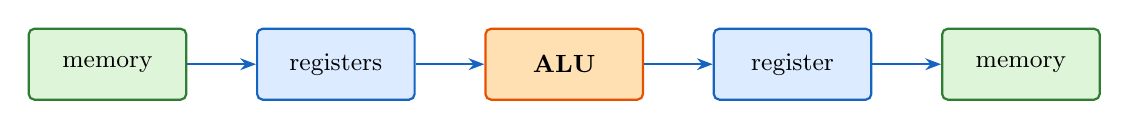
\begin{tikzpicture}[x=10mm, y=10mm]
        \node[memblk, minimum width=20mm] (m1)  at (0,0)   {memory};
        \node[blk,    minimum width=20mm] (r1)  at (2.9,0) {registers};
        \node[cpublk, minimum width=20mm] (alu) at (5.8,0) {ALU};
        \node[blk,    minimum width=20mm] (r2)  at (8.7,0) {register};
        \node[memblk, minimum width=20mm] (m2)  at (11.6,0){memory};
        \draw[flow] (m1) -- (r1);
        \draw[flow] (r1) -- (alu);
        \draw[flow] (alu) -- (r2);
        \draw[flow] (r2) -- (m2);
    \end{tikzpicture}
    \end{center}

    \vspace{2mm}
    {\small The register set is not an abstract list. It is the set
    of places where your variables must \alert{physically be} before
    the ALU can touch them.}
\end{frame}

\begin{frame}[plain]{The APSR Condition Flags}
	\begin{center}
	\begin{tikzpicture}[x=4.6mm, y=4.6mm]
		\foreach \bit/\lbl/\hl in {%
			31/N/1, 30/Z/1, 29/C/1, 28/V/1, 27/Q/0,
			26/{}/0, 25/{}/0, 24/{}/0, 23/{}/0, 22/{}/0, 21/{}/0, 20/{}/0,
			19/{}/0, 18/{}/0, 17/{}/0, 16/{}/0,
			15/T/0, 14/{}/0, 13/{}/0, 12/{}/0,
			11/{}/0, 10/{}/0, 9/{}/0, 8/{}/0, 7/{}/0, 6/{}/0, 5/{}/0, 4/{}/0,
			3/{}/0, 2/{}/0, 1/{}/0, 0/{}/0}{
			\pgfmathtruncatemacro{\col}{31-\bit}
			\ifnum\hl=1
				\node[cell, fill=primary!18, draw=primary, font=\tiny\ttfamily\bfseries,
				      minimum width=4.4mm, minimum height=4.4mm]
				      at (\col,0) {\lbl};
			\else
				\node[cell, fill=Gray!12, draw=Gray!45, text=Gray!70, font=\tiny\ttfamily,
				      minimum width=4.4mm, minimum height=4.4mm]
				      at (\col,0) {\lbl};
			\fi
		}
		\node[lbl, anchor=north, font=\scriptsize] at (2,-0.5) {condition flags};
		\node[lbl, anchor=north, font=\scriptsize, text=Gray] at (22,-0.5) {execution state --- not covered here};
	\end{tikzpicture}
	\end{center}
	\vspace{2mm}
	\begin{center}
		{\small
			\striped
			\begin{tabular}{@{}c l R{.56\textwidth}@{}}
				\toprule
				\textbf{Bit} & \textbf{Flag} & \textbf{Set when} \\
				\midrule
				31 & \textbf{N} Negative & Bit~31 of the result is 1 (negative when interpreted as signed) \\
				30 & \textbf{Z} Zero & The result is exactly zero (set by a \texttt{CMP} of equal values) \\
				29 & \textbf{C} Carry & Unsigned addition produced a carry, or unsigned subtraction did \emph{not} borrow \\
				28 & \textbf{V} Overflow & A signed operation exceeded the representable range \\
				\bottomrule
		\end{tabular}}
	\end{center}
	\vspace{2mm}
	{\small \textbf{This is how a processor makes decisions:} the C statement \texttt{if (x == y)} works by subtracting, throwing away the difference, and testing the \textbf{Z} flag. \textbf{C} is the carry-out of the final full adder. \textbf{V} is the XOR of the carries into and out of the MSB. These are circuits you have already built.}
\end{frame}

\begin{frame}[plain]{The Generic ARMv7-M Memory Map}
	\begin{columns}[c]
	\begin{column}{.52\textwidth}
		\begin{center}
		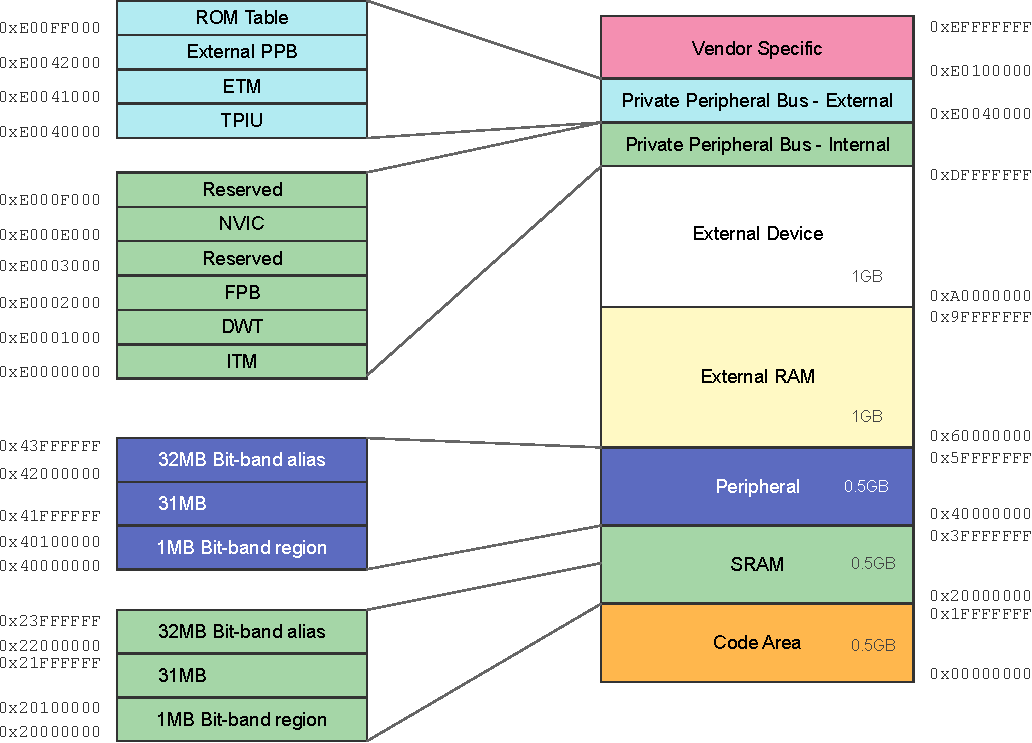
\includegraphics[width=\textwidth, height=.7\textheight, keepaspectratio]{assets/m4-memory-map.pdf}
		\end{center}
	\end{column}
	\begin{column}{.44\textwidth}
		{\small\emph{This is the map defined by ARM.}}

		\vspace{2mm}
		ARM defines a \alert{standardized} address space shared by every Cortex-M core. This is what lets code move between chips from different vendors.

		\vspace{2mm}
		The space is 4\,GB wide, split into sub-regions, each with its own separate role.

		\vspace{2mm}
		{\small
		\striped
		\begin{tabular}{@{}l l@{}}
			\toprule
			\textbf{Base} & \textbf{Region} \\
			\midrule
			\texttt{0x0000\,0000} & Code --- 512\,MB \\
			\texttt{0x2000\,0000} & SRAM --- 512\,MB \\
			\texttt{0x4000\,0000} & Peripheral --- 512\,MB \\
			\texttt{0x6000\,0000} & External RAM --- 1\,GB \\
			\texttt{0xA000\,0000} & External device --- 1\,GB \\
			\texttt{0xE000\,0000} & Private peripheral bus \\
			\bottomrule
		\end{tabular}}
	\end{column}
	\end{columns}
\end{frame}

\begin{frame}{The Regions That Matter to You}
	{\small\emph{Most of that 4\,GB does not matter to us. These are the regions you need to remember.}}

	\vspace{1mm}
	\begin{columns}[T]
	\begin{column}{.48\textwidth}
		\textbf{Code area} (512\,MB)
		{\small
		\begin{itemize}\itemsep1pt
			\item Maps to Flash: program code and constant data
			\item Also holds the bootloader and the \alert{interrupt vector table}
			\item Code executes directly from Flash
		\end{itemize}}
		\vspace{1mm}
		\textbf{SRAM} (512\,MB)
		{\small
		\begin{itemize}\itemsep1pt
			\item Variables, the stack, dynamic data
			\item Faster to access than Flash
		\end{itemize}}
	\end{column}
	\begin{column}{.48\textwidth}
		\textbf{Peripheral} (512\,MB)
		{\small
		\begin{itemize}\itemsep1pt
			\item The memory-mapped registers of every on-chip peripheral --- GPIO, timers, ADC, DAC, UART, SPI, I\textsuperscript{2}C
			\item Each peripheral gets its own address range
		\end{itemize}}
		\vspace{1mm}
		\textbf{Private peripheral bus}
		{\small
		\begin{itemize}\itemsep1pt
			\item System peripherals: \alert{NVIC}, SysTick, MPU
			\item Debug and trace: DWT, ITM, FPB
		\end{itemize}}
	\end{column}
	\end{columns}

	\vspace{3mm}
	\begin{block}{On your STM32F446RE}
		512\,KB of Flash and 128\,KB of SRAM fill only a small part of the regions above. The rest of the map is \alert{reserved}, not missing. Reading an address with nothing there causes a HardFault.
	\end{block}
\end{frame}

\begin{frame}[plain]{The 4\,GB Memory Map}{The STM32F446RE inside it}
	\begin{center}
		\begin{tikzpicture}[x=10mm, y=7mm]
			\tikzset{
				pop/.style  = {draw=primary, fill=primary!12, thick},
				mem/.style  = {draw=secondary, fill=secondary!12, thick},
			}
			% ---- LEFT: the whole 4 GB, to scale ----
			\def\lx{0}\def\lw{1.4}\def\ltop{6.0}\def\lbot{0}
			\node[lbl, anchor=south, align=center, font=\scriptsize\bfseries]
			at ({\lx+\lw/2},{\ltop+0.2}) {The whole\\4\,GB space};
			\draw[draw=Gray, fill=white, thick] (\lx,\lbot) rectangle ({\lx+\lw},\ltop);
			\foreach \frac/\nm in {0.031/Flash, 0.125/SRAM, 0.250/peripherals, 0.875/private}{
				\pgfmathsetmacro{\y}{\lbot+\frac*(\ltop-\lbot)}
				\draw[pop] (\lx,\y) rectangle ({\lx+\lw},{\y+0.12});
				\node[lbl, anchor=west, font=\scriptsize] at ({\lx+\lw+0.12},{\y+0.06}) {\nm};
			}
			\node[lbl, anchor=east, font=\scriptsize\ttfamily] at ({\lx-0.1},\ltop) {0xFFFFFFFF};
			\node[lbl, anchor=east, font=\scriptsize\ttfamily] at ({\lx-0.1},\lbot) {0x00000000};
			\node[lbl, anchor=north, align=center, font=\scriptsize] at ({\lx+\lw/2},{\lbot-0.25})
			{almost all of it\\is empty};
			% ---- RIGHT: what is actually populated ----
			\def\rx{5.6}\def\rw{4.2}\def\rh{0.66}
			\node[lbl, anchor=south, align=center, font=\scriptsize\bfseries]
			at ({\rx+\rw/2},{\ltop+0.2}) {What the F446RE actually populates};
			\foreach \i/\addr/\nm/\sz/\hl in {%
				0/{0xE000 E000}/{Private peripherals}/{NVIC, SysTick, debug}/1,
				1/{0x4002 3800}/{AHB1}/{RCC, GPIOA--GPIOH}/1,
				2/{0x4001 0000}/{APB2}/{USART1, ADC1, SYSCFG, EXTI}/1,
				3/{0x4000 0000}/{APB1}/{TIM2--TIM5, USART2, SPI2, I\textsuperscript{2}C}/1,
				4/{0x2000 0000}/{SRAM}/{128 KB --- variables, stack}/0,
				5/{0x0800 0000}/{Flash}/{512 KB --- code, constants}/0}{
				\pgfmathsetmacro{\y}{\ltop-0.5-\i*(\rh+0.16)}
				\ifnum\hl=1
				\draw[pop] (\rx,\y) rectangle ({\rx+\rw},{\y-\rh});
				\else
				\draw[mem] (\rx,\y) rectangle ({\rx+\rw},{\y-\rh});
				\fi
				\node[anchor=west, font=\scriptsize\bfseries] at ({\rx+0.1},{\y-\rh/2+0.15}) {\nm};
				\node[lbl, anchor=west, font=\scriptsize] at ({\rx+0.1},{\y-\rh/2-0.16}) {\sz};
				\node[lbl, anchor=east, font=\scriptsize\ttfamily] at ({\rx-0.1},{\y-\rh/2}) {\addr};
			}
			\draw[decorate, decoration={brace, amplitude=4pt}, draw=primary]
			({\rx+\rw+0.15},{\ltop-0.5-1*(\rh+0.16)}) --
			({\rx+\rw+0.15},{\ltop-0.5-3*(\rh+0.16)-\rh});
			\node[lbl, anchor=west, align=left, font=\scriptsize, text=primary]
			at ({\rx+\rw+0.4},{\ltop-0.5-2.4*(\rh+0.16)})
			{every address\\here begins\\\texttt{0x4\ldots}};
		\end{tikzpicture}
	\end{center}
	\vspace{1mm}
	{\small\centering \emph{Now let's see where the real STM32 resources live.} ARM \alert{fixes} this layout for every Cortex-M device. This is why the NVIC sits at the same address on every vendor's chip. Reading an empty region causes a \alert{HardFault}. This is why a wild pointer crashes loudly, instead of failing quietly.\par}
\end{frame}

\begin{frame}[plain]{Byte Order: Endianness}
	\begin{center}
		\begin{tikzpicture}[x=10mm, y=8mm]
			% ---- the 32-bit value, split into four bytes ----
			\node[lbl, anchor=east] at (1.05,4.5) {the value};
			\foreach \i/\b in {0/0x12, 1/0x34, 2/0x56, 3/0x78}{
				\draw[draw=primary, fill=primary!12, thick]
				(1.2+\i*0.95,4.15) rectangle (1.2+\i*0.95+0.9,4.85);
				\node[font=\scriptsize\ttfamily] at (1.2+\i*0.95+0.45,4.5) {\b};
			}
			\node[lbl, anchor=west, font=\scriptsize] at (5.1,4.5) {\texttt{0x12345678}};
			\node[lbl, font=\scriptsize, text=primary] at (1.65,3.75) {most significant};
			\node[lbl, font=\scriptsize, text=primary] at (4.1,3.75) {least significant};
			% ---- shared address axis down the middle ----
			\draw[-{Stealth[length=2mm]}, draw=Gray] (3.6,2.6) -- (3.6,0.2);
			\node[lbl, anchor=south, rotate=90, font=\scriptsize] at (3.12,1.4)
			{increasing address};
			\foreach \i in {0,...,3}{
				\pgfmathsetmacro{\y}{2.1-\i*0.62+0.275}
				\node[lbl, font=\scriptsize\ttfamily, anchor=west] at (3.72,\y)
				{\ifcase\i Addr\or Addr+1\or Addr+2\or Addr+3\fi};
			}
			% ---- the two conventions ----
			\foreach \xo/\name/\ba/\bb/\bc/\bd in {%
				0.35/{Big-endian}/0x12/0x34/0x56/0x78,
				4.75/{Little-endian}/0x78/0x56/0x34/0x12}{
				\begin{scope}[shift={(\xo,0)}]
					\node[lbl, anchor=south, align=center] at (1.35,2.75) {\textbf{\name}};
					\foreach \i/\byte in {0/\ba, 1/\bb, 2/\bc, 3/\bd}{
						\pgfmathsetmacro{\y}{2.1-\i*0.62}
						\draw[draw=secondary, fill=secondary!12, thick]
						(0.9,\y) rectangle (1.8,\y+0.55);
						\node[font=\scriptsize\ttfamily] at (1.35,\y+0.275) {\byte};
					}
				\end{scope}
			}
			\node[lbl, anchor=north, align=center, text=primary] at (1.7,0.0)
			{MS byte at the\\lowest address};
			\node[lbl, anchor=north, align=center, text=primary] at (6.1,0.0)
			{LS byte at the\\lowest address};
		\end{tikzpicture}
	\end{center}
	\vspace{1mm}
	{\small\centering Both conventions store the \alert{same four bytes}. They only differ in which end sits at the lowest address. The Cortex-M4 is \alert{little-endian}, like x86, so raw memory dumps look the same on the target and on a typical PC.\par}
\end{frame}

\begin{frame}{Summary: Can You Now Explain\ldots}
	{\small
	\begin{enumerate}\itemsep3pt
		\item What does ``32-bit'' mean at each of the three architectural layers --- ISA, microarchitecture, platform?
		\item Why is ARM described as a \textbf{load-store RISC} architecture, and what does that force every C statement like \texttt{x = x + 1;} to cost?
		\item Why does Cortex-M use a \textbf{short pipeline} and no cache, rather than chasing peak throughput?
		\item What are \textbf{SP}, \textbf{LR} and \textbf{PC} used for, and which bits of \texttt{xPSR} does every \texttt{if} and loop rest on?
		\item How does a C statement reach a \textbf{peripheral register}, given that the \textbf{4\,GB memory map is fixed by ARM}?
	\end{enumerate}}
	\vspace{2mm}
	\begin{block}{Next: Chapter 3 --- Memory, Addressing and Pointers}
		If a peripheral is just an address, then a pointer is how C reaches it.
	\end{block}
\end{frame}

%===============================================================================
\section{Design Challenge}
%===============================================================================
\begin{frame}{Design Challenge}{To be worked on paper, before any code}
    \leavevmode
    {\small\emph{We now use this chapter's performance model to make a processor-selection decision.}}

    \vspace{2mm}
    \begin{block}{The brief}
        You are choosing a processor for a motor controller. It must run a control loop 20\,000 times per second. Each pass through the loop needs about 180 instructions.
    \end{block}
    \vspace{2mm}
    {\small Using the CPU-time equation, find the minimum clock frequency needed if the processor averages 1.3 cycles per instruction. Then calculate what fraction of the CPU that loop uses at 16\,MHz, at 48\,MHz, and at 180\,MHz. Decide which of the three frequencies you would choose, and explain the safety margin you leave. Finally, state what you would need to measure to check whether the 1.3 CPI assumption is realistic.}
\end{frame}

\begin{frame}[plain]
    \begin{center}
        \vfill
        {\usebeamerfont{title}\color{primary}\Huge Questions?}
        \vfill
        {\small\color{Gray} \emph{Introduction to ARM Cortex-M Microprocessors} --- Chapter 2}
        \vfill
    \end{center}
\end{frame}
\end{document}